\chapter{Measurements}
This section will discuss three experiments that characterize the CKIDs on the Device Chip. 

\section{Cryostat}
The chip has been mounted in the cryostat called the ADR because of it's cooling mechanism. Adiabatic Demagnetization refriguratior.It is shown in Fig. \hl{Insert image}

\begin{figure}[ht]
	\centering
	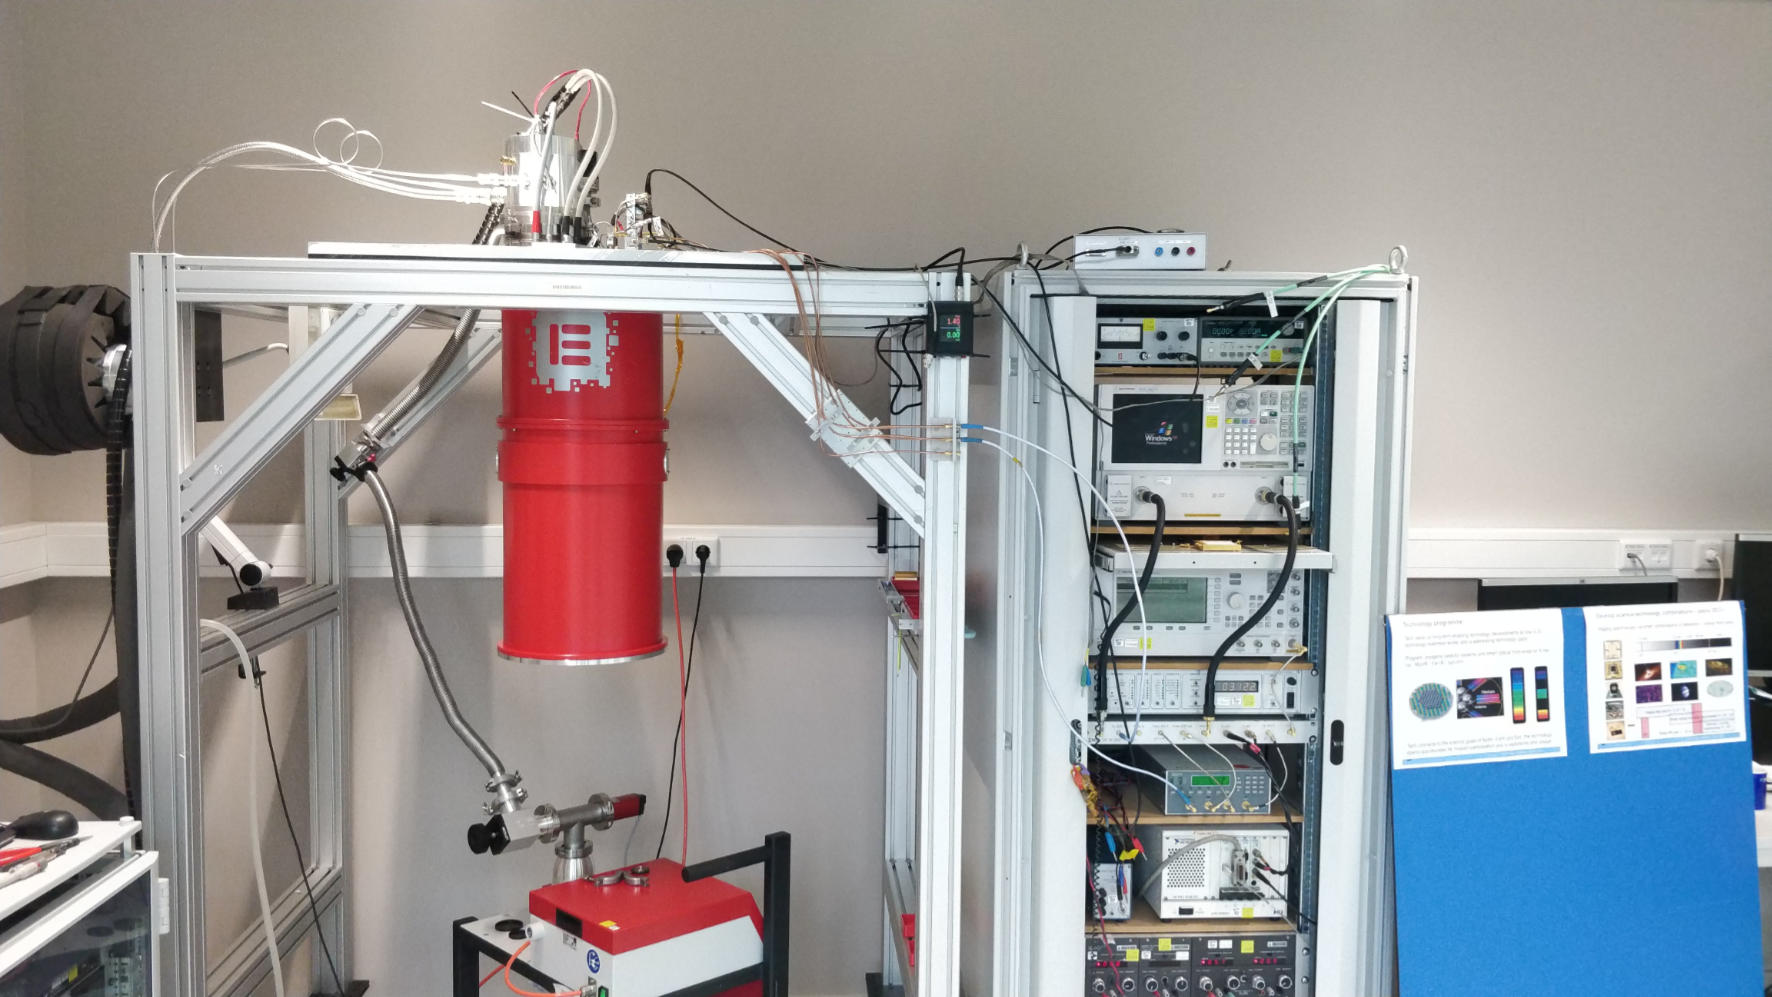
\includegraphics[width=.70\linewidth]{figures/ch5_measurement/ADR_OverviewV1.jpg}
	\caption{\hl{Describe image cryostat.}}
	\label{fig:ch6_ADR_image}
\end{figure}

This cryostat uses a Matroska doll design in which there is a large cylindrical vessel that forms the first cooling stage that cools to 50K. In this cylindrical vessel, a second heatshield in which a second Pulse tube stage cools to 3K. Inside the 3K stage, are two plates with two Adiabatic Demagnetization salt tubes that cool to 800mK, and the final plate cools to 120mK temperature.

A scematic representation of the parts of the cryostat are given in Fig. \hl{ref figure}

\begin{figure}[h!!!!!!!!!!]
	\centering
	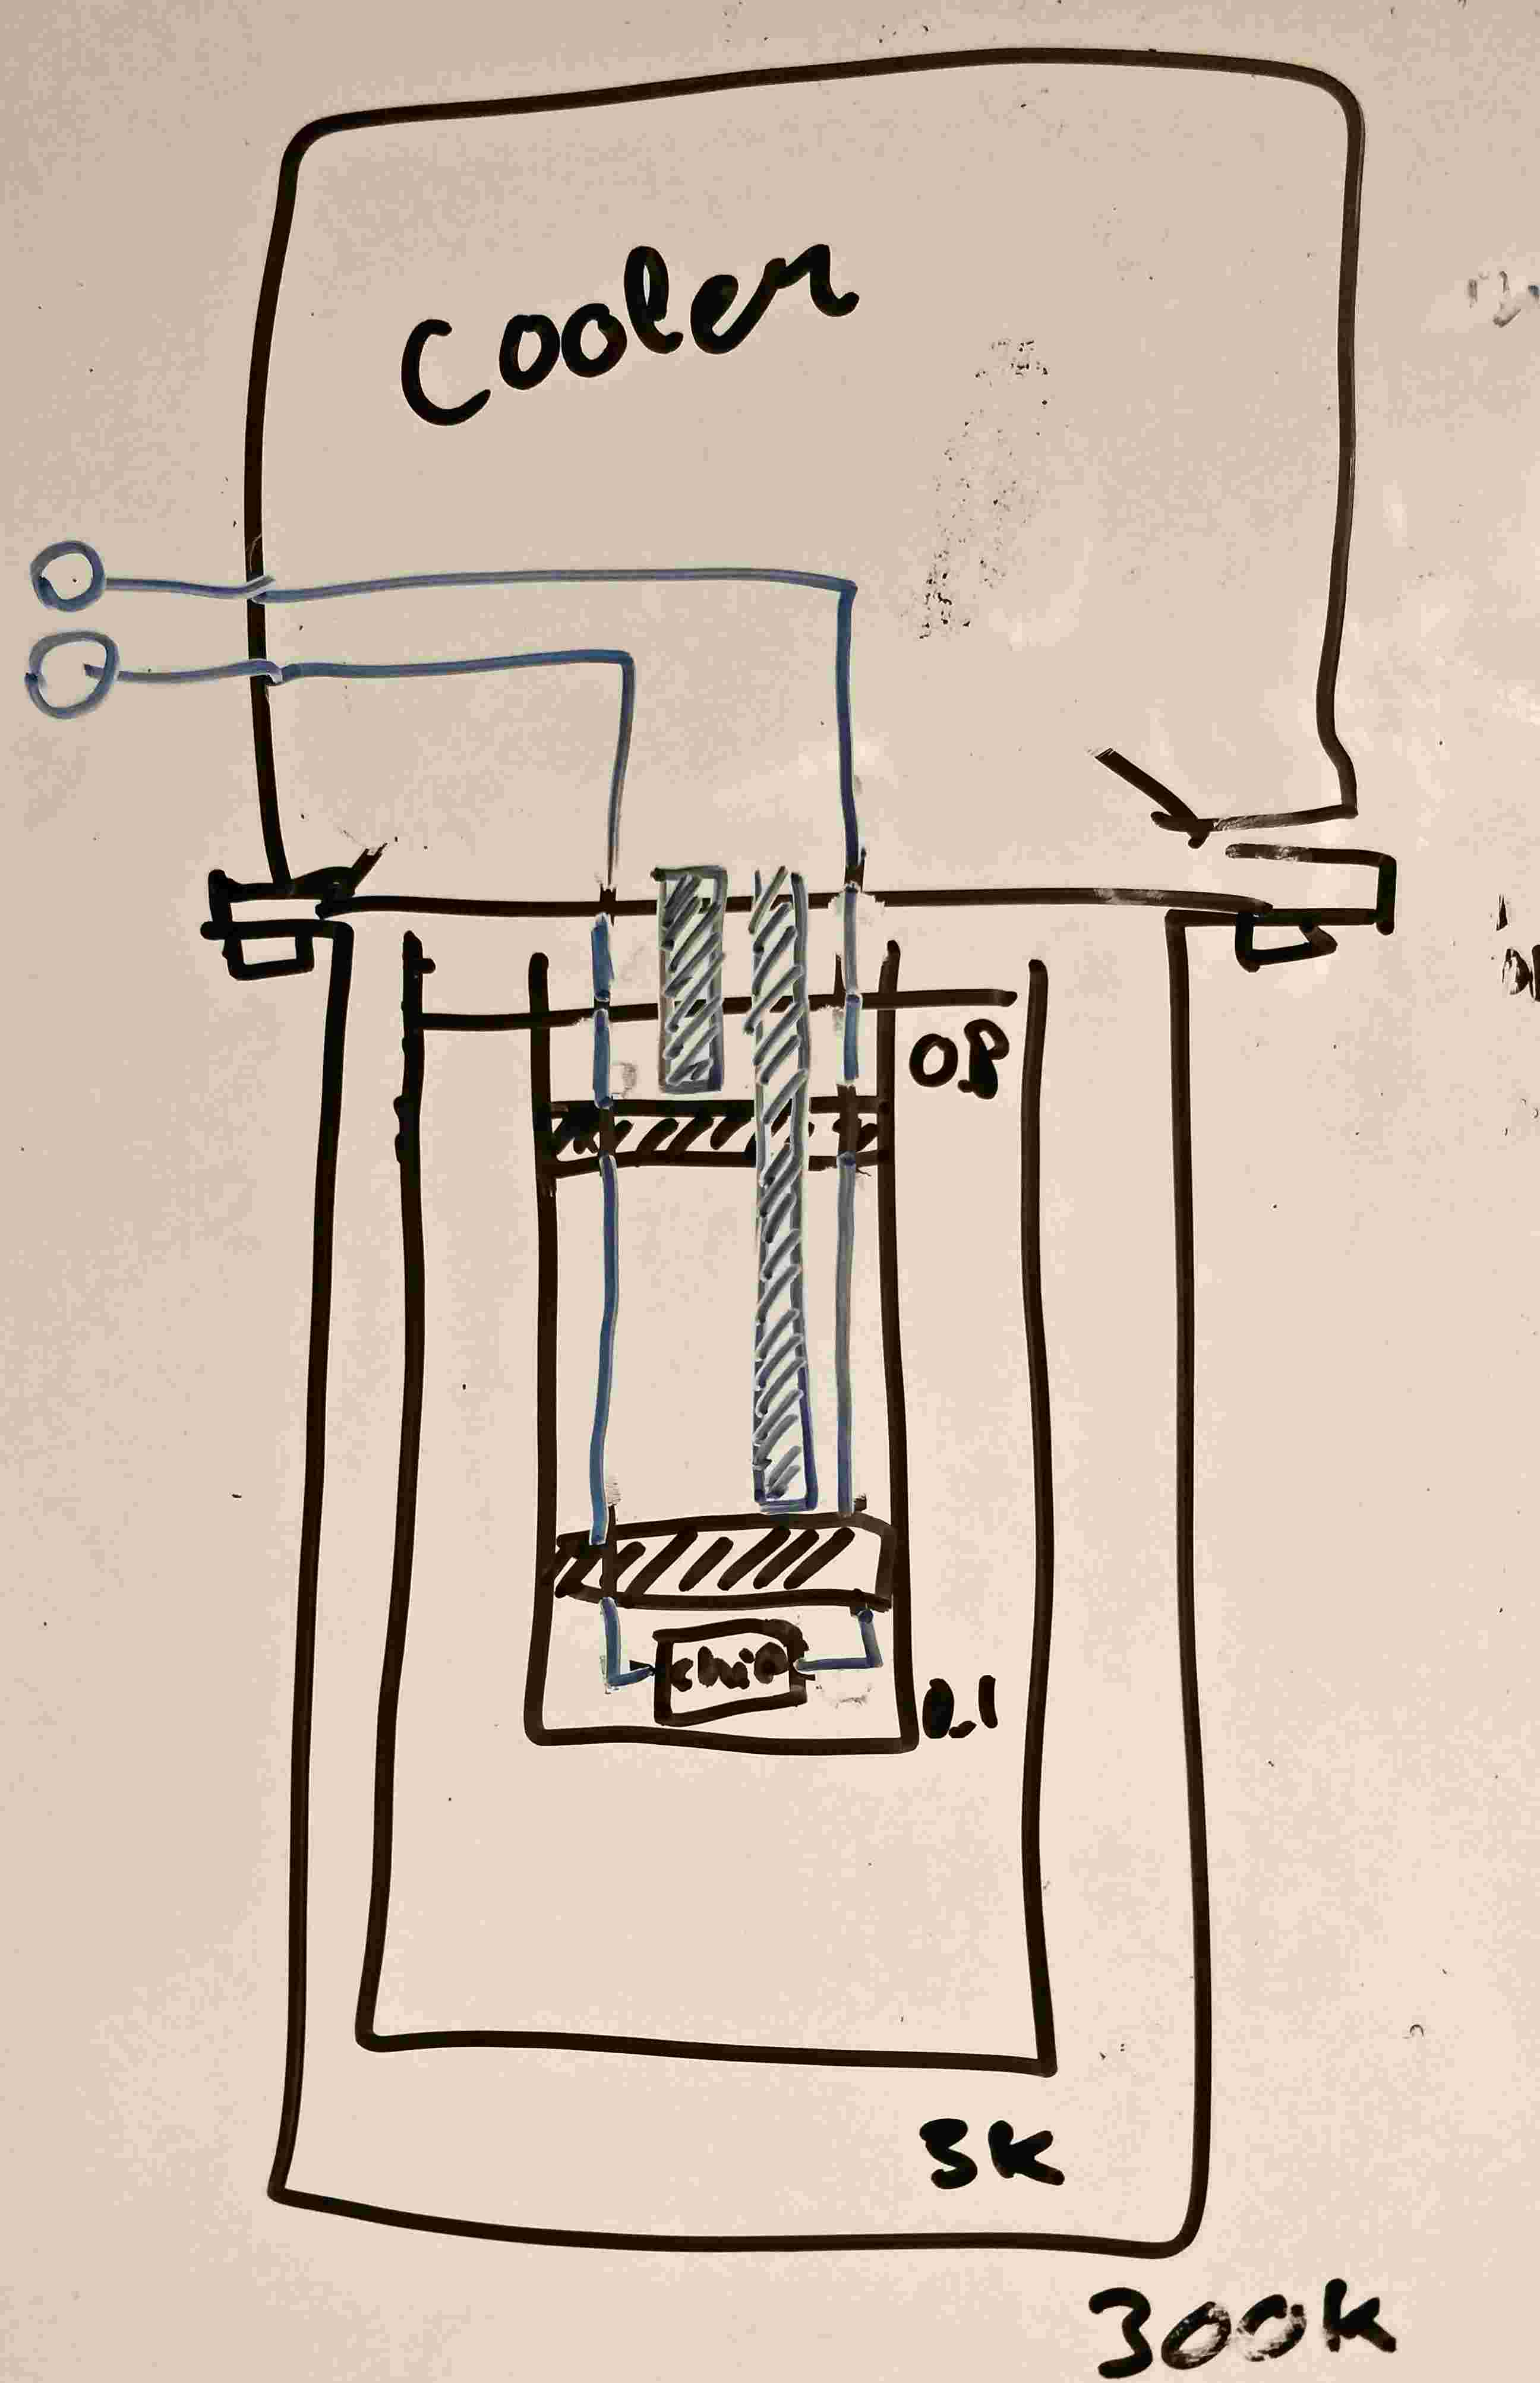
\includegraphics[width=.40\linewidth]{figures/ch5_measurement/Cryostat_scematicV2.jpg}
	\caption{\hl{Describe image cryostat.}}
	\label{fig:ch6_cryostat_scematic}
\end{figure}

For all these experiments, the chip is mounted in a so-called Box-in-box configuration, as shown in the dissertation of \cite{devisserVisser2014Quasiparticle2014}. Care is taken to avoid any Light of frequencies higher than the gap freq of aluminum entering the chip holder.

The temperature of 120mK has been chosen because the hold time for the system is longer(~1.5 day) when the temperature is higher\cite{devisserVisser2014Quasiparticle2014}. This is a comprimize between GR-noise contribution and hold-time.

\FloatBarrier
\section{Method: Exp.1 - VNA}
\label{sec:M_VNA}
\hl{Reference Source:} \cite{devisserReadoutpowerHeatingHysteretic2010}
A vector network analyzer (VNA) is a measurement device that generates a sweeping tone(~GHz) between two frequencies for characterizing the device under test(DUT) to determine the transmission properties of the DUT. After the sweep we can see a trace of $|S_{21}|$ and $arg(S_{21})$

In our case, we want to use the VNA to determine the resonance frequency, optimal readout frequency, and Quality factors of the CKIDs on the chip. With the VNA we will first do a sweep of the approximate frequency range in which we expect the $F_0$ of the set of CKIDs to be. This is the range of 5.5 to 6.5 GHz.

When we found the approximate location of the resonance frequencies we want to reduce the sweep range to see one CKID dip in detail. Then after determining the $|S_{21}|$ a Lorentzian can be fitted to this curve to obtain $Q_c$ and $Q_i$.

The step of determining the Quality factors is repeated for all readout powers from -120dBm upward in steps of 4dBm until we see that the Lorentzian dip gets skewed as can be seen in \cite{devisserReadoutpowerHeatingHysteretic2010}

\hl{TODO: make scematic image about whole setup!}
\hl{Reference Source:}

%\subsection{Dataset}


\section{Results: Exp.1 - VNA}
\hl{TODO:}
\section{Discussion on Exp.1 - VNA: F0, Qc, Qi}
\section{Method: Exp.2 - PSD}

%\subsection{Describe setup}

%\subsection{What is done and recorded}

%\subsection{Dataset}
The dataset used to do the PSD analysis is 
%\subsection{How is it analyzed.}


\hl{Reference Source:}

In the previous experiment in section \ref{sec:M_VNA} the resonance frequencies for the optimal readout power have been detemined.\\ 

In this experiment we will use the found resonace frequencies to set up a single tone readout at the frequency $F_0$ of one of the CKIDs shunted resonace frequency. That CKID is then the current KID under test. 

The generated signal is split into two parts. One part is fed into the cryostat and is then attenuated by the various \hl{passifisation} stages that prevent 'hot' electrons from heating up the final stage of the cryostat which than does not reach the target temperature.

When the signal passes through the chip the KID under test will modulate the amplitude and phase of the signal. The important takeaway here is that The GR-noise and TLS noise processes of the KID will change the resonace frequency of the KID under test. Thus these noise processes modulate the signal and after the signal has passed the KID under test both noise sources have been encoded into the signal in the form of the aplitude and phase modulation of the signal.

The first step after the signal leaves the chip is that a HEMT amplifier($T_{noise}~3-4K$\cite[p.83]{devisserVisser2014Quasiparticle2014}) at the 3K stage is used to amplify the signal by $\sim$ 35dB\cite[p.83]{devisserVisser2014Quasiparticle2014}. Because the gain of this first stage is high the HEMT amplifier determines almost exclusivly the noise propeties of the total system.\cite[Eq 8.37]{couchDigitalAnalogCommunication2013}

When the signal leaves the cryostat it is mixed using an IQ-mixer with an attenuated version of the signal from the signal generator which is illustrated in Fig. \ref{} The resulting baseband signal is digitized using an ADC so that the timestream of the Aplitude and phase can be determined.
The welch method is employed to obtain a direct PSD of this signal.
\begin{figure}[ht]
	\centering
	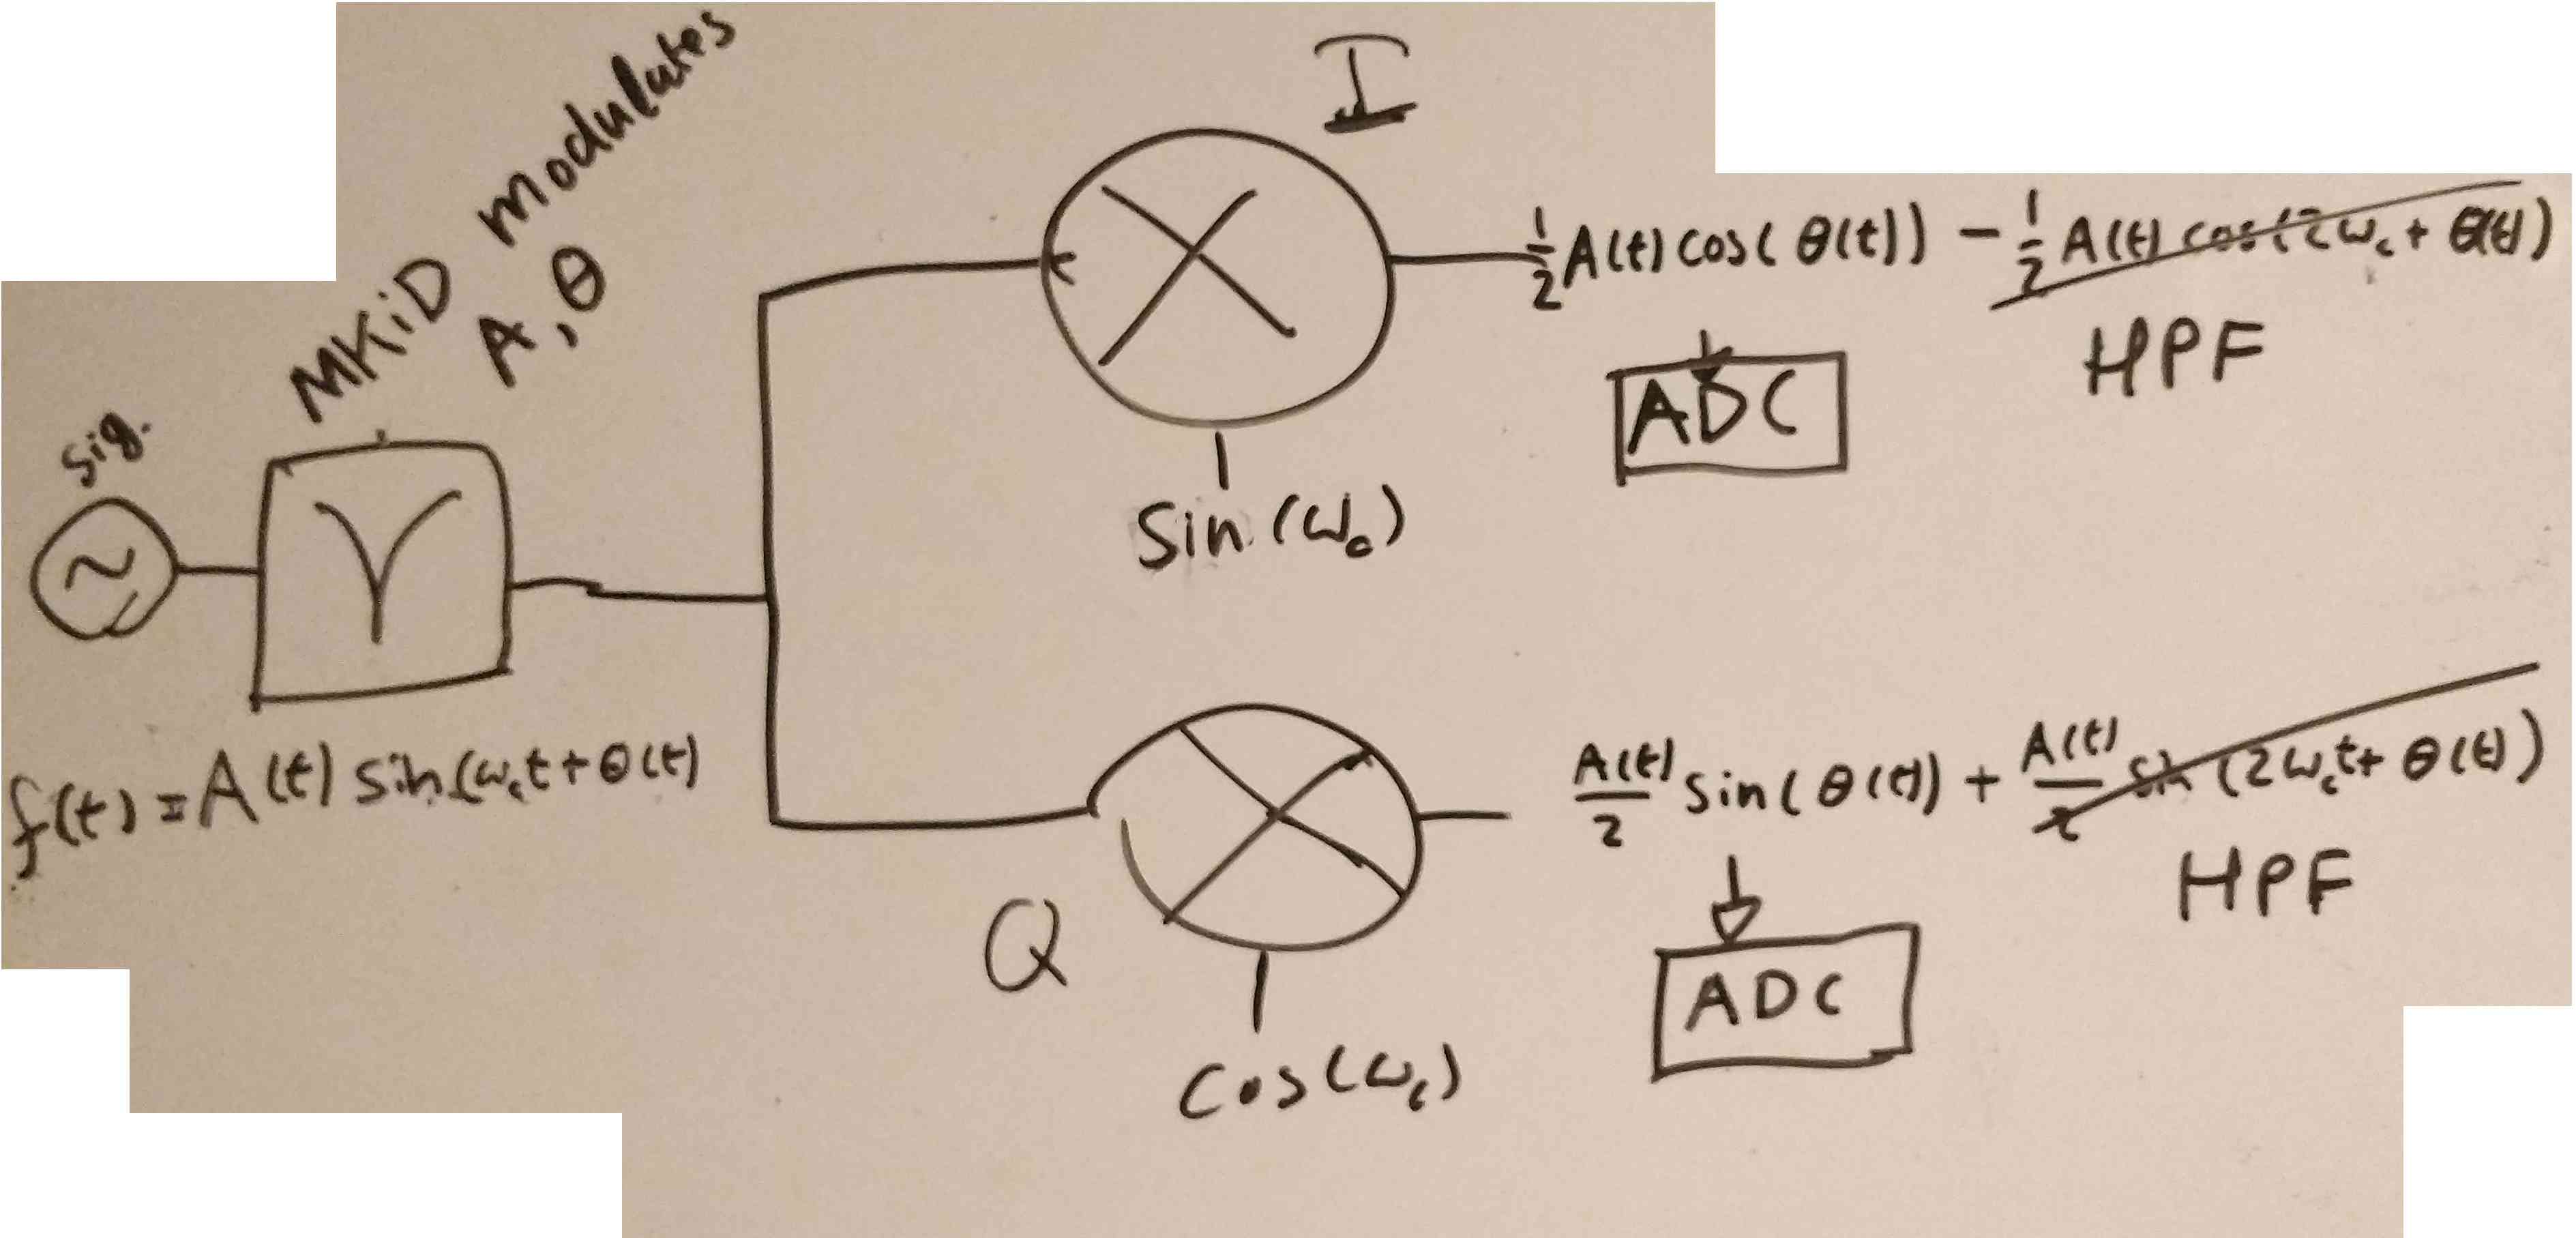
\includegraphics[width=.80\linewidth]{figures/ch5_measurement/PSD_IQmixing_overview_Edit.jpg}
	\caption{An overview is shown of the simplified signal chain. A readout tone is generated on the left. Then the signal is fed into the cryostat into the chip. The noise in the MKID modulates the amplitude and the phase of the readout tone as a function of time. This modulates the readout tone on the readout frequency. an IQ mixer is used to retrieve the In-phase and Quadrature(90 deg out of phase) components in the signal. This signal is then fed into a High-Pass filter that removes all the high frequency components and is subsequently fed into a Analog-to-digital converter. In the data processign software a PSD is calculated.  }
	\label{fig:ch6_Signal_overview}
\end{figure}




\section{Results: Exp.2 - PSD}
\subsection*{preliminary analysis}
\hl{preliminary results!!! while i am at it i might better write it down.}


\textbf{Slope TLS noise:}
TLS noise is given in general by 
\begin{equation}
	S_{\theta,TLS}(f) = C(P_{read})\frac{1}{\sqrt{f}}
\end{equation}
So we want to know what the slope is of this in log-log plot. 
so first we want to make the function not a variable of f but of $f=10^{x}$
So we obtain 
\begin{equation}
	S_{\theta,TLS,log}(x) = C(P_{read})\frac{1}{\sqrt{10^{x}}}
\end{equation}
And then take the $10log_{10}(...)$ of the whole function:
\begin{equation}
	S_{\theta,TLS,log-log}(f) = 10log(C(P_{read})\frac{1}{\sqrt{10^{x}}})
\end{equation}
split..
\begin{equation}
	S_{\theta,TLS,log-log}(f) = 10log(C(P_{read}))+10log(10^{-0.5x})
\end{equation}
Which then simplifies to 
\begin{equation}
	S_{\theta,TLS,log-log}(f) = C_{1}-5x
\end{equation}
Which means that TLS noise has a slope in log-log plot of 5dB per decade!

\textbf{Readout noise:}
From Eq. \ref{eq:ch2_Readout_noise} we can obtain the noise line that the readout circuit gives.
from \cite{devisserVisser2014Quasiparticle2014} we know that the $T_{noise} \sim 7K$

\begin{equation}
	S_{\theta} = \frac{4*1.38E-23*7}{10^{-3-\frac{86}{10}}} = 1.53\cdot 10^{-10} 
\end{equation}
In dB by doing $10*log_{10}(1.53E-10)$
$$10*log_{10}(1.53E-10) = -98 dBc/Hz$$


\begin{figure}[ht]
	\centering
	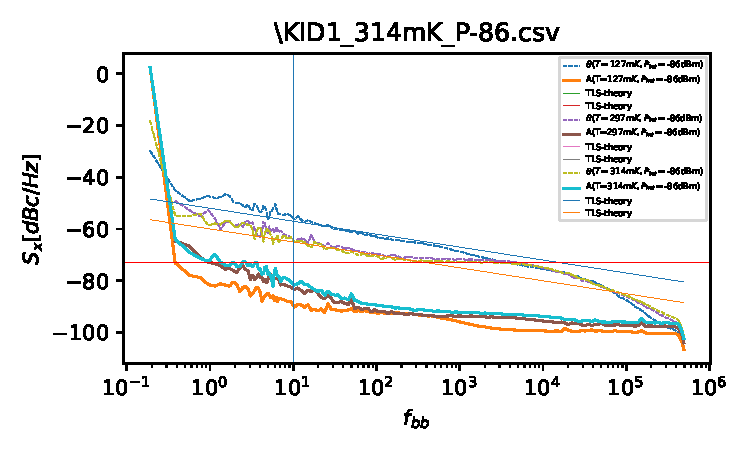
\includegraphics[width=.95\linewidth]{figures/ch5_measurement/KID1_127mK_P-86KID1_297mK_P-86KID1_314mK_P-86.pdf}
	\caption{KID1:}
	\label{fig:First_results}
\end{figure}

\hl{My Jochem stitch code seems to explain the GR noise level! Look into if it is ok!}
\section{Discussion on Exp.2 - PSD}


\section{Method: Exp.3 - Dark NEP}
\hl{TODO: temperature variation.}
\hl{TODO: write about DC measurement}

\section{Results: Exp.3 - dark NEP}

\begin{equation}
    NEP_{elec}(f) = \frac{\sqrt{S_{x}(f)}}{\frac{\eta_{qp}\tau_{qp}}{\Delta} \frac{dX}{dN_{qp}}} \sqrt{(1+(2\pi f \tau_{qp})^{2})(1+(2\pi f \tau_{ring})^{2})} 
    \label{eq:ch3_elecNEPdef}
\end{equation}
\begin{equation}
    \frac{dx}{dP_{dark}} = \frac{\eta_{pb}\tau_{qp} (T)}{\Delta(0)}\frac{dx}{dN_{qp}(T)}
    \label{eq:ch3_res_dark}
\end{equation}
The overall dependency flowchart is given in Fig. \ref{}
\begin{figure}[ht]
	\centering
	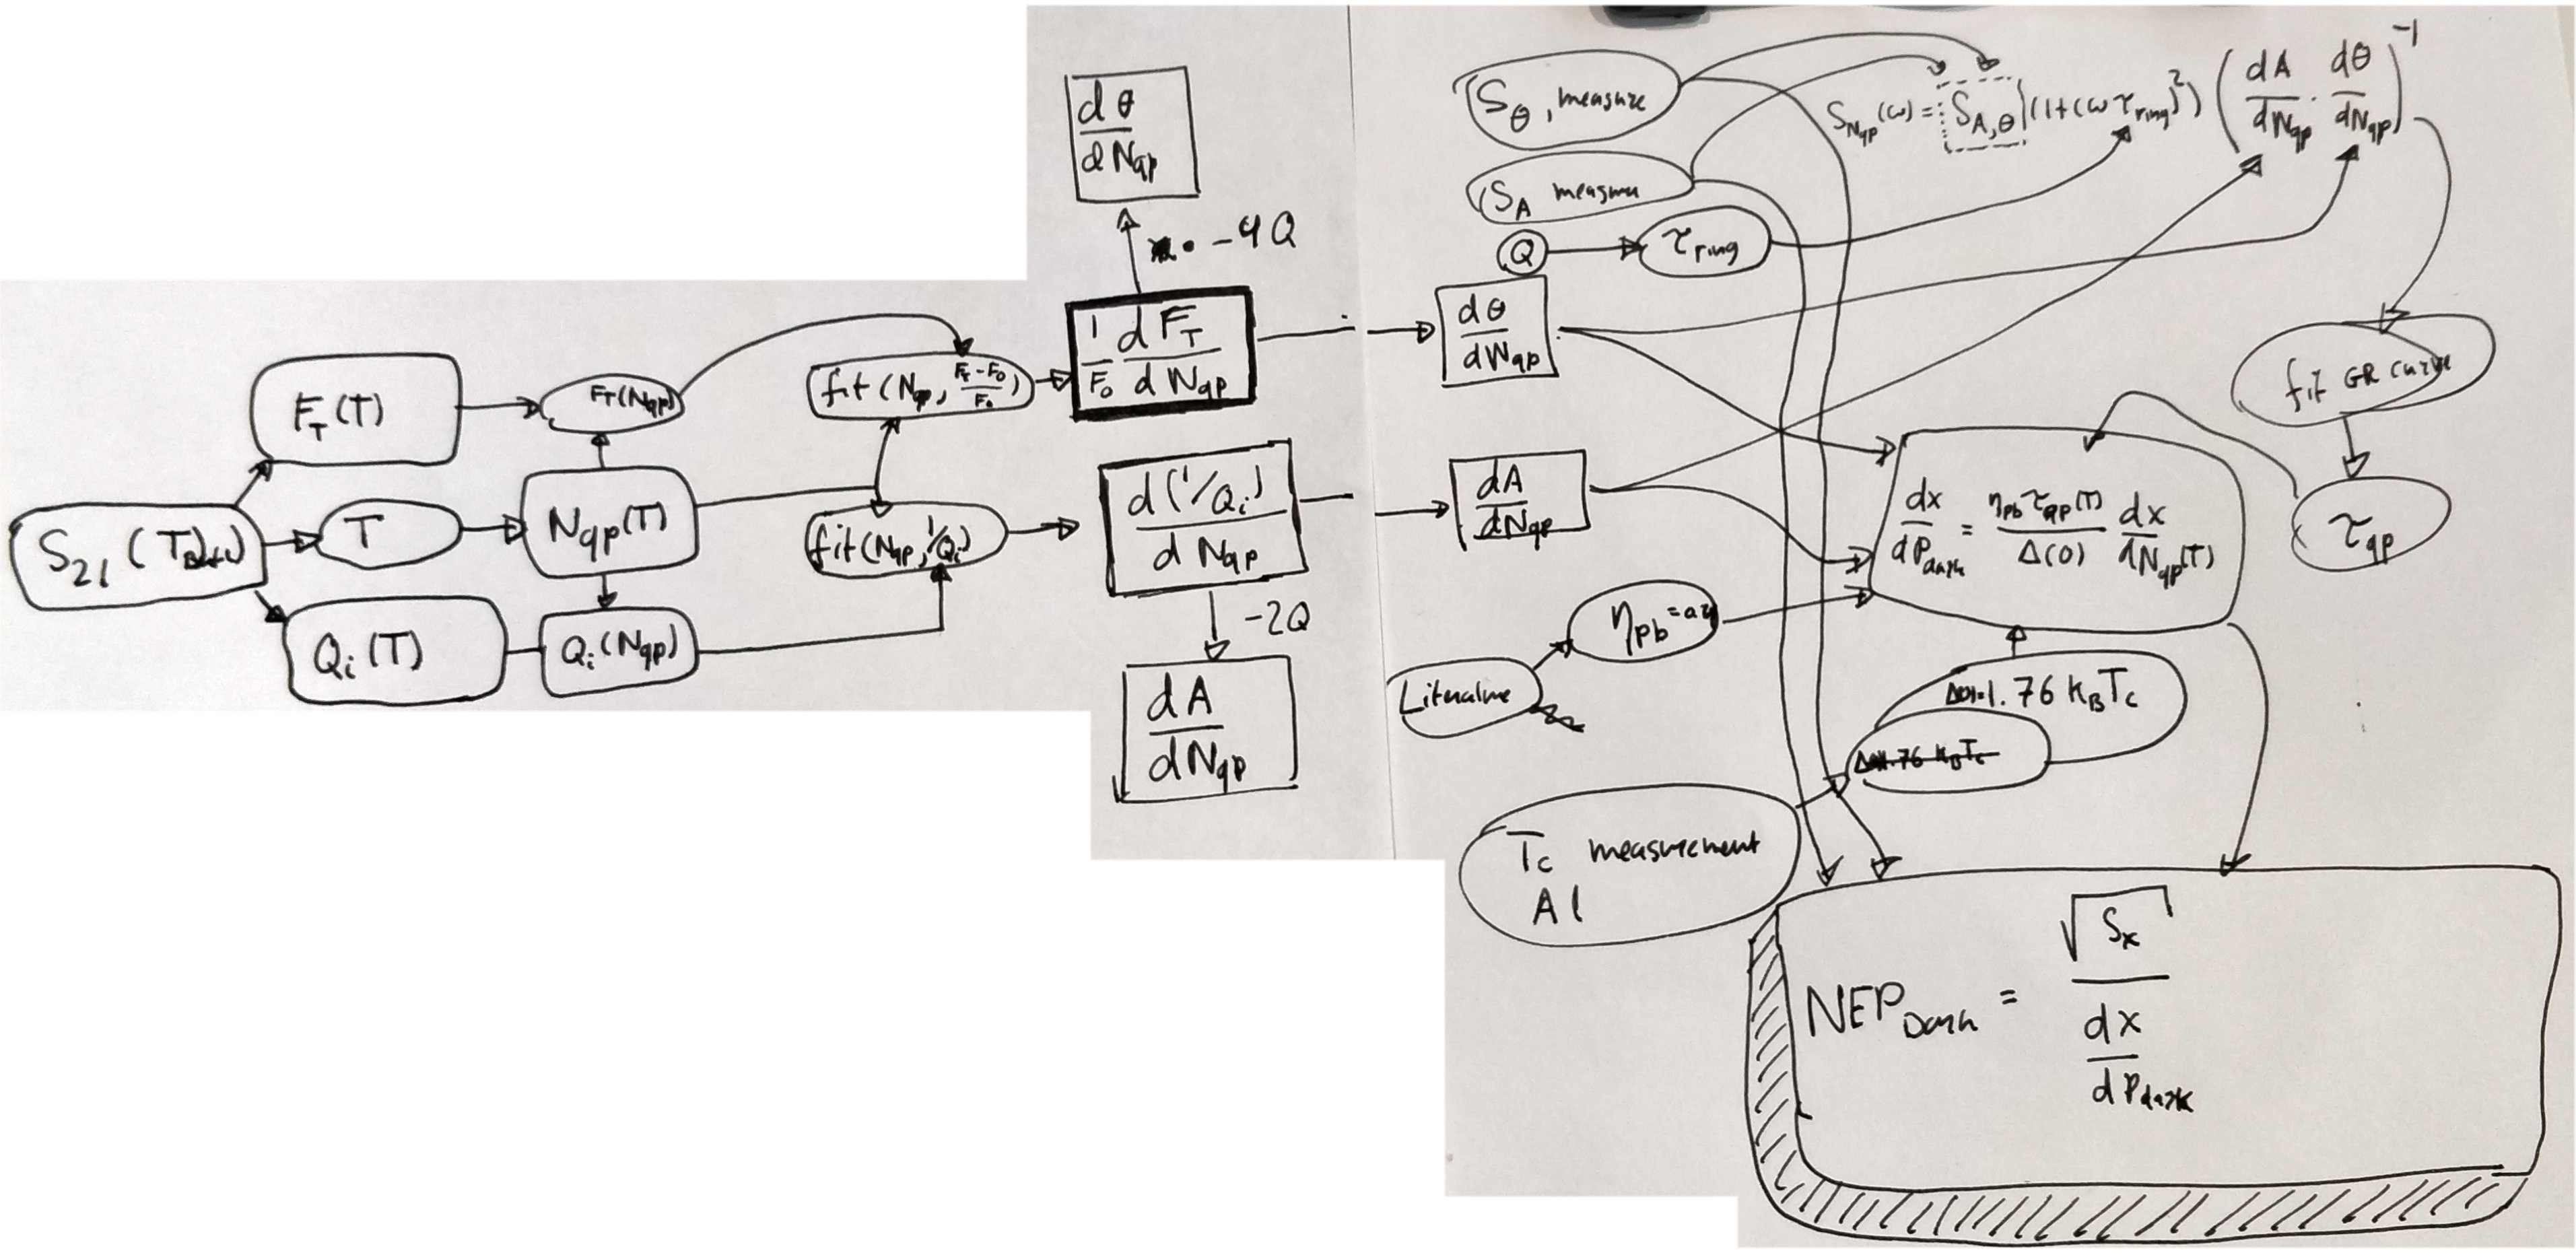
\includegraphics[width=.80\linewidth]{figures/ch5_measurement/Overview_Process.jpg}
	\caption{An overview is shown of the of how all parameters depend on eachother and how they should be obtained.}
	\label{fig:NEP_flow_diagram}
\end{figure}



\subsection*{Checking Popt.}
First we want to check if Popt is ok! Because if it is not then we are in trouble because the relation between the phase and the incident radiation becomes nonlinear.
This is shown in the following Fig. \ref{fig:Popt_KID1}\ref{fig:Popt_KID2}\ref{fig:Popt_KID3}
\begin{table}[ht]
    \centering
    \begin{tabular}[t]{lccc}
    \hline
    KID\# & $ P_{opt} (dBm) $ & $ \sim F_{0}$ (Graph) & Supected KID \\
    \hline
    1 & -94 & 4.9083 & C7G3\\
   	2 & -90 & 5.0762 & C9G3 \\
    3 & -94 & 5.5424 & C8G3 \\
	4 & -87 & 5.8222 & C10G4 \\
    5 & -92 & 5.9134 & C11G4 \\
    6 & -87 & 6.0052 & C12G4 \\
    \hline
    \end{tabular}
    \caption{Table with optimal readout powers. You can judge from the skewness of the $S_{21}$ dip and the Lowpass charateristic that you have overdriven the MKID into non-linear regime. The second is the suspected MKID number based on only the C9G3 MKID had a piece on Hybrid CPW which explains the higher readout freq.}
    \label{tab:}
\end{table}%


\begin{figure}[h!!!!!]
	\centering
	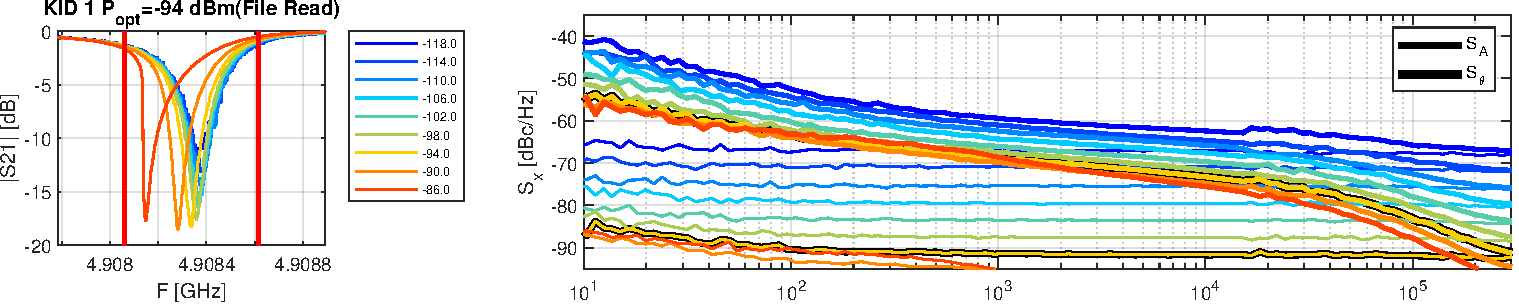
\includegraphics[width=\linewidth]{figures/chA_Appendix/Popt_KID1.pdf}
	\caption{asdfffffffdsa}
	\label{fig:Popt_KID1}
\end{figure}

\begin{figure}[h!!!!!]
	\centering
	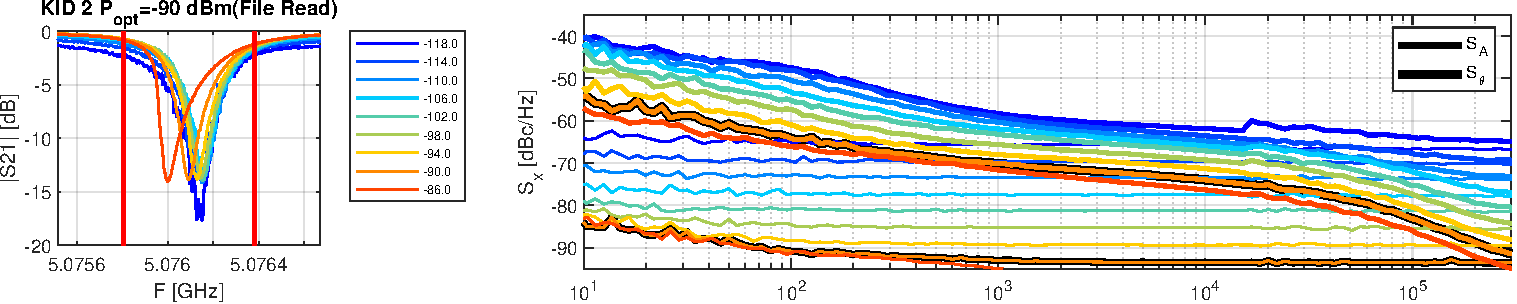
\includegraphics[width=\linewidth]{figures/chA_Appendix/Popt_KID2.pdf}
	\caption{asdffdsa}
	\label{fig:Popt_KID2}
\end{figure}

\begin{figure}[h!!!!!]
	\centering
	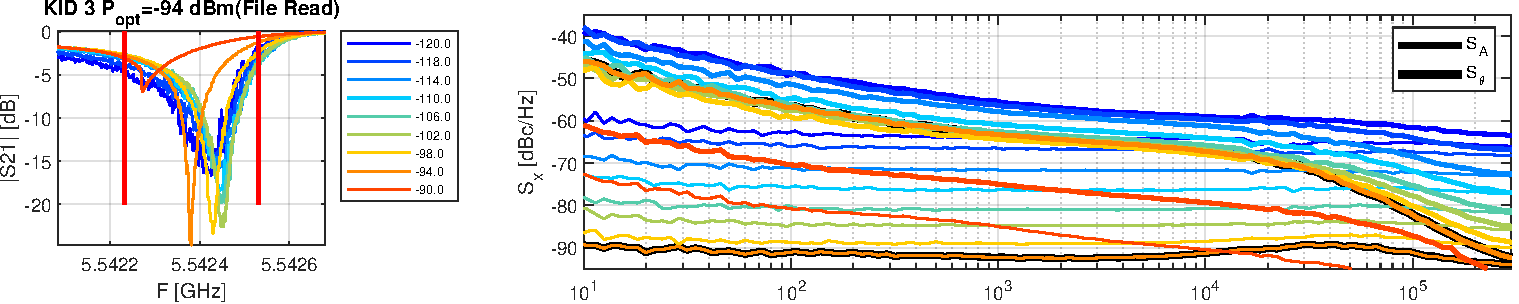
\includegraphics[width=\linewidth]{figures/chA_Appendix/Popt_KID3.pdf}
	\caption{asdffdsa}
	\label{fig:Popt_KID3}
\end{figure}

\begin{figure}[h!!!!!]
	\centering
	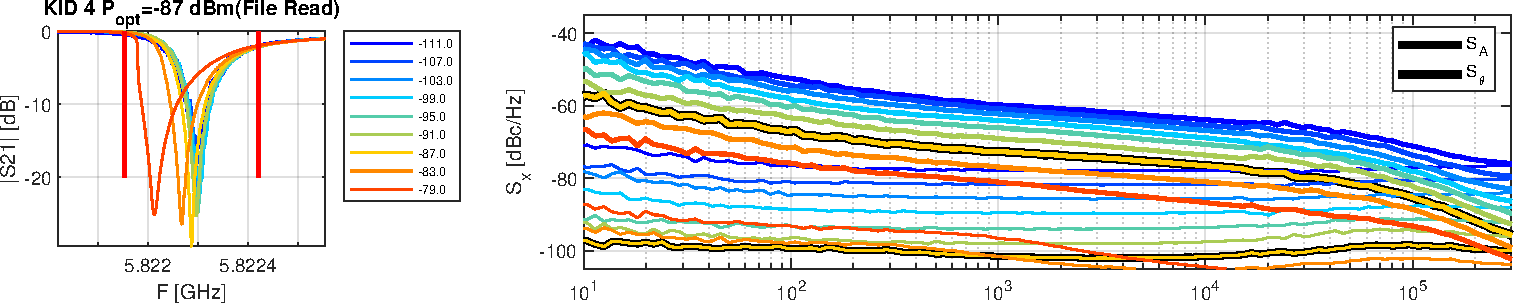
\includegraphics[width=\linewidth]{figures/chA_Appendix/Popt_KID4.pdf}
	\caption{asdffdsa}
	\label{fig:Popt_KID4}
\end{figure}
asdfaf
\begin{figure}[h!!!!!]
	\centering
	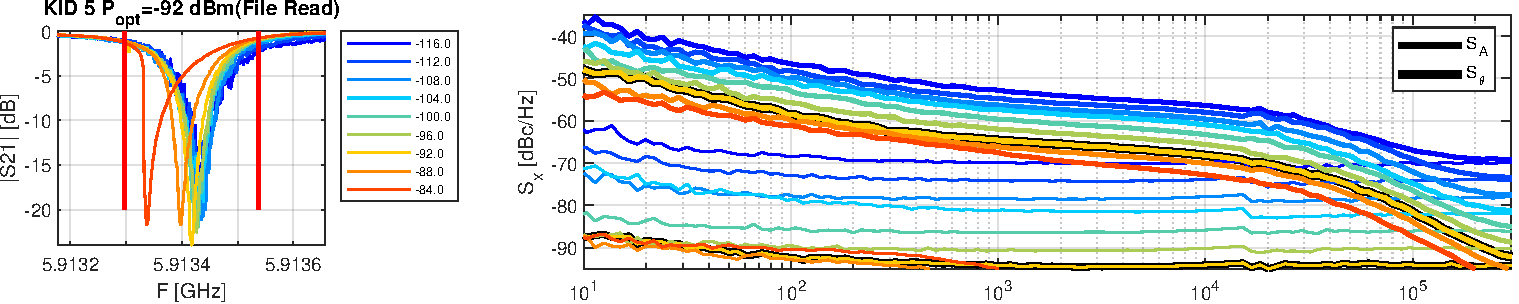
\includegraphics[width=\linewidth]{figures/chA_Appendix/Popt_KID5.pdf}
	\caption{asdffdsa}
	\label{fig:Popt_KID5}
\end{figure}
\begin{figure}[h!!!!!]
	\centering
	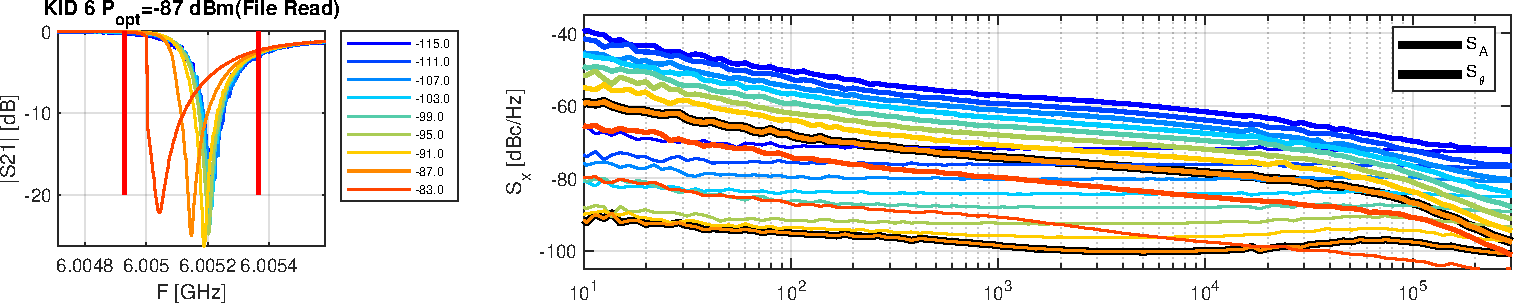
\includegraphics[width=\linewidth]{figures/chA_Appendix/Popt_KID6.pdf}
	\caption{asdffdsa}
	\label{fig:Popt_KID6}
\end{figure}


\FloatBarrier

\subsection*{Find S21 dips for all temperatures and Powers.}
\textbf{Find the following expressions (In code):}
\cite{janssenEquivalenceOpticalElectrical2014}
\begin{equation}
    \frac{F_{T}(T)-F_{0}}{F_{0}} \textrm{  Vs.  } T
\end{equation}
\begin{equation}
    \frac{1}{Q_{i}(T))} \textrm{  Vs.  } T
\end{equation}


\begin{enumerate}
	\item Find all dips in S21 data for all temperatures and T
\end{enumerate}


\subsection*{Convert T to $N_{qp}$}

\begin{figure}[ht]
	\centering
	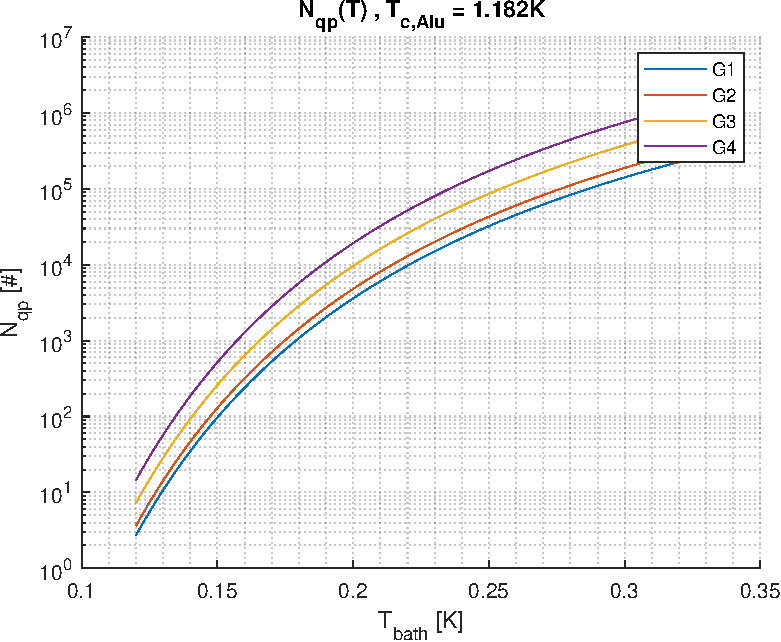
\includegraphics[width=\linewidth]{figures/ch5_measurement/N_qp_funcT.pdf}
	\caption{Relation between the bath temperature and $N_{qp}$. Code based on getNqp\_Tbath.m function. Author: J.Baselmans}
	\label{fig:}
\end{figure}

\subsection*{Determine $\tau_{qp} $with cross power spectral density - fitting}
Workflow is as follows:
\begin{enumerate}
	\item (Done)Find $P_{opt}$ with Noiseanalysis\_PdepV7.m
	\item (Done)Find all PSD curves with Noiseanalysis\_2DV1.m
	\item (Done)Use TDanalysisV2.m to find CrossPSD
	\item (Working)Find offset of TLS-noise spectrum.
	\item Remove TLS noise spectrum by subtracting in normal domain
	\item Use CrossPSDJBV2.m to fit $\tau_{qp}$
\end{enumerate}
\textbf{How to remove offset}
First we want to know the offset from lets say 1Hz
That is then the value for $C_{TLS,Cross-PSD,dB}$. I don't know yet if this will be the same as $C_{TLS}$. I don't think so. 

Once $C_{TLS,Cross-PSD}$ is found we can put it in the formula:
$$S_{TLS} = 10^{C_{TLS,Cross-PSD,dB}/10}f^{-0.5}$$
Then we obtain the following in the limit that Readout noise is \textbf{Low!}
$$S_{GR,lin} = 10^{\frac{S_{CrossPSD}}{10}} - 10^{C_{TLS,Cross-PSD,dB}/10}f^{-0.5}$$





\subsection*{other parameters and fill in to obtain dark responsivity}

\subsection*{Obtain PSD.}

The 2D PSD files are contained In
%\directory{C:/Users\siets\Dropbox\Universiteit\Natuurkunde\MEP\Simulations\Matlab\ADR\Data\analysis\LT254\Data\Analysis\scripts\ADR\Data\LT254\Sietse\LT254\Sietse\Chip11\Noise\vs\T\FFT\\2D\Noise\_2D.mat}
%\directory{C:/Users/siets/Dropbox/Universiteit/Natuurkunde/MEP/Simulations/Matlab/ADR/Data/analysis/LT254/Data/Analysis/scripts/ADR/Data/LT254/Sietse/LT254/Sietse/Chip11/Noise/vs/T/FFT//2D/Noise/_2D.mat}
\directory[bslash]{X:\DIR\SUBDIR}

\subsection*{dark NEP plots}


\section{Discussion on Exp.3 - dark NEP} 



\end{document}